%\documentclass[a4paper,11pt]{article}
\documentclass[apj, onecolumn]{emulateapj}
\usepackage[utf8x]{inputenc}
%\usepackage[pdftex]{graphicx}
%\usepackage[L1]{fontenc}
\usepackage{amsfonts,amsmath,amssymb,amstext}
\usepackage{enumerate}
\usepackage{hyperref}
\usepackage{placeins}
\usepackage{listings}
\usepackage{url}
\usepackage{natbib}
\bibliographystyle{apj}
\title{CALIFA growth curve photometry}
%\author{Simona Bekerait\.{e}, sbekeraite@aip.de}
\begin{document}
\maketitle
\section*{Motivation for having independent photometry measurements}

As CALIFA sample was selected from the SDSS survey, all the CALIFA galaxies have SDSS Petrosian magnitudes  (TODO: cite Blanton 2001, Yasuda). However, SDSS Petrosian magnitudes are designed to capture a fixed percentage of the total flux which depends on the galaxy profile. As shown in \cite{Blanton2001}, the Petrosian flux measurement of a large exponential disk includes virtually all the flux, however, the ratio between the total flux and the Petrosian flux of a galaxy with de Vaucouleurs profile is only $\approx$80\%. Moreover, the SDSS Petrosian radii are based on signal-to-noise-ratio of the image, therefore flux in bands with low S/N (u, z) is underestimated, possibly affecting photometric stellar mass models.\\

The CALIFA survey is primarily diameter-limited and consists of galaxies with quite large (40-80\") SDSS isophotal radii. The SDSS DR7 pipeline (TODO: cite) does not always perform well for bright, large galaxies, over-subtracting the sky or picking child photometric components for total flux measurements. Besides, all images contain foreground and background objects (stars, background galaxies, cosmic rays, image artifacts) that, if not accounted for, contribute to the error in both flux and sky value measurements. Just masking nuisance objects would lead to systematic underestimation of the galaxy magnitude, because the galaxy areas under them would remain excluded from the total flux measurement.

\section*{Image preparation}
Neglecting the flux from the masked regions would lead to systematic underestimation of galaxy brightness. Simple interpolation would not have been applicable, so we chose a procedure known as inpainting -- masked pixels were iteratively replaced with a Gaussian inverse-distance weighted average of the neighbouring real pixels, starting with the pixels with the largest number of nearest neighbours. In order to apply the masks provided by the collaboration and available for r band images to the other 4 SDSS bands, we measured the shift between the different images and their r band counterparts using their WCS (FITS World Coordinate System) $\alpha$ and $\delta$ coordinates, then shifted the masks and cropped the images accordingly.

A small number of galaxies with large masked regions are distorted and were flagged as such. In such cases, only flux from non-masked regions was included.

\section*{The procedure}

Surface photometry of galaxies is made difficult due to the fact that galaxies are extended objects without clear outer edges. Various methods have been used to measure the galaxy magnitudes, including 2D modelling of galaxy images, signal-to-noise based methods (Petrosian magnitudes, \cite{Petrosian1976}, \cite{Strauss2002}), measuring flux inside a radius limited by surface brightness, using fixed apertures, etc.

Growth curve of a galaxy is the profile of integrated magnitude shown as a function of the radius of the current aperture\cite{Okamura1999}, which can be elliptical in general case. If the sky is subtracted accurately, this profile flattens asymptotically as the flux from the galaxy drops to zero. In a perfect case, the cumulative flux at the end of such a profile corresponds to the total flux of the galaxy.

In theory, growth curve photometry measurements are superior to the other methods mentioned, retrieving the flux of all types of galaxy profiles well and making no prior assumptions or applying arbitrary cutoffs in surface brightness level, S/N level or aperture size. It is sensitive to even small flux levels at the outskirts of galaxies. In addition, it does not depend on the global features of the image, measuring the sky level in the immediate vicinity of the galaxy. The local sky values are more accurate than the sky mean frequently used for sky subtraction, resulting in better sky subtraction and more accurate magnitudes. It is also testable, because the shapes of the growth curves reveal inaccurate sky subtraction or interloping objects. 

Trade-off between systematic errors correlated with galaxy light distribution (like SDSS Petrosian quantities) and random errors (due to masking).

Our implementation of a growth curve photometry algorithm first measures the sky value by constructing a mean flux-per-pixel profile in 1 px wide ellipses with given position angles, axis ratios, and major axis values). We use per-pixel values so as to avoid dependence on geometry, i.e. the ellipse shape, distance from the center, parts of galaxies which are outside the image frame.

We assume that flux falls off asymptotically until it is indistinguishable from the sky fluctuations.
If we were fitting the slope of the mean flux per pixel profile in sufficiently wide rings, the best fit line should become horizontal at some radius, which we might then consider the edge of the galaxy. In practice this is not the case, given that incomplete masks, light from the other objects and sky gradients make the best fit slope switch from negative to slightly positive at some point. 

We fit 150 px wide annuli of the flux profile using linear regression, going outwards in steps of 10 px. When the flux profile slope becomes non-negative, we take the mean of the unmasked pixels in the current annulus as the sky value, and the ellipse with major axis value at the middle of the ring as the galaxy's edge. We use the photometric galaxy center from SDSS DR7 as the starting point and position angles from light-moments fitting by the collaboration. Three colour-composite images of all the galaxies were inspected by eye and either the SDSS isophotal axis ratio or the light-moments fit axis ratio was selected visually. 

We have checked that this procedure gives quite good results and is robust even in the presence of large masked regions or faint unmasked objects. %The sky values obtained were consistently lower than a simple mean of the image outside the galaxy and SDSS sky values provided in image headers (quantify!!).  

In the second step we construct two growth curves for each galaxy - the sky subtracted cumulative flux profiles for all pixels and unmasked pixels. In the majority of cases they do flatten, showing that the sky subtraction was accurate. Then we calculate the magnitudes using the standard prescription given at \url{http://www.sdss.org/dr7/algorithms/fluxcal.html#counts2mag}

\subsection{Outliers and quality flags}
In several cases the growth curve procedure did not work well, either producing artificially large flux values due to incomplete masking of the foreground, or missing some of the flux because of being too close to the frame border. In the first case, we used flux from non-masked pixels only, after checking that we do not lose a large fraction of the flux near the center of the galaxy. 


\section{Error estimation}
\subsection{Magnitude errors}
First of all we estimate the error in counts as described in \url{http://www.sdss.org/dr7/algorithms/fluxcal.html#counterr}. The number of counts provided in the corrected SDSS frames is related to the number of photo-electrons counted by the CCDs via the inverse gain, provided with the SDSS frames:

\begin{equation}
photo-electrons = counts * inverse gain
\end{equation}

The contributions of the dark current and read noise are included too via the following expression:

\begin{equation}
error_{count} = \sqrt([counts+sky]/inverse\ gain + Npix*(dark\ variance + sky error))
\end{equation}

Here $error_{count}$ is the count error, counts+sky is the sum of the counts within the galaxy without sky subtraction, Npix is the number of pixels within the galaxy and dark variance is the total noise caused by dark current and read noise and provided by the SDSS pipeline. We used the difference between sky values for all pixels and unmasked pixels only as the sky error value:

\begin{equation}
sky_{err} = sky - skyM
\label{sky_err}
\end{equation}

Note that eq.\ref{sky_err} only accounts for the Poissonian error in counts. To estimate the uncertainties due to sky subtraction, we add the difference between sky-subtracted flux and the same flux with $sky + sky_{err}$ subtracted:

\begin{equation}
err_{skySub} = \mod{(all counts\ -\ sky*Npix) - (all\ counts\ -\ (sky-sky_{err})*Npix)}
\label{sky_err}
\end{equation}

In order to roughly estimate the influence of masked foreground objects we also add half of the difference between sky-subtracted counts of all pixels and unmasked pixels only:

\begin{equation}
count_{diff} = \frac{1}{2}(all\ counts\ -\ sky*Npix)\ -\ (all\ countsM - skyM*NpixM))
\end{equation}

\begin{equation}
total\ error = \sqrt{error_{count}} + \frac{1}{2} count_{diff} + err_{skySub}
\end{equation}

Finally, the apparent magnitude uncertainty is calculated as shown at \url{http://www.sdss.org/dr7/algorithms/fluxcal.html#counts2mag}:

\begin{equation}
error(mag) = 2.5 / ln(10) * total\ error / counts
\end{equation}

\subsection{Half light semi-major axis and 90\% light radii errors}

The main contribution to the uncertainty of these two quantities comes from errors in sky subtraction and masking errors. The former contributes to the total flux profile, whereas the latter is provided by the photometry pipeline as the difference between masked and non-masked half-light radii. We add them too.


\FloatBarrier
\section*{Tests}
We filled blank image with real sky from one of the CALIFA SDSS images (140). We selected a large patch of sky outside the previously determined limit of the galaxy. The mean value of the empty sky was 122.93 counts with $\sigma$ = 5.4 counts.

We created fake galaxies with GALFIT, using de Vaucouleur's profile (n = 4) and an exponential disk. Its r magnitude was equal to 12.76 mag, half-light radii of both profiles were set equal to 45 px, the axis ratio b/a = 0.5. 

The recovered sky value for an exponential profile was 123.01 counts, for a deVaucouleur profile -- 123.22 counts. The recovered magnitudes were 12.77 mag and 12.88 respectively, differing from the input ones by 0.01 and 0.12 mag. To put in in other way, the measured fluxes differed from the models by 1.2\% and 9.7\%. These errors dropped to 0.01\% and 3\% for small simulated galaxies (having half light radii equal to 14 px), for which the sky could have been estimated more accurately.


\begin{figure}[h]
\centering
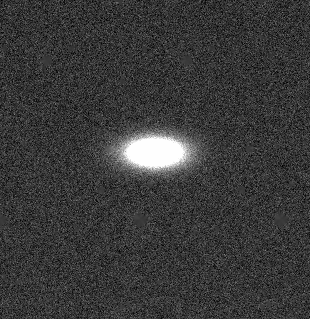
\includegraphics[scale=0.6]{img/test_expDisk}
\caption{Simulated galaxy with an exponential profile.}
\label{fig:test}
\end{figure}


\section*{Results}

The growth curve magnitudes in the 5 SDSS bands are brighter than the SDSS Petrosian magnitudes by 0.79, 0.39, 0.35, 0.35 and XX mag respectively. 

%On average, our sky values were smaller than SDSS sky values by 0.16 ADU (for ~650 galaxies with SDSS sky values in their headers).
\begin{figure}[h]
\centering
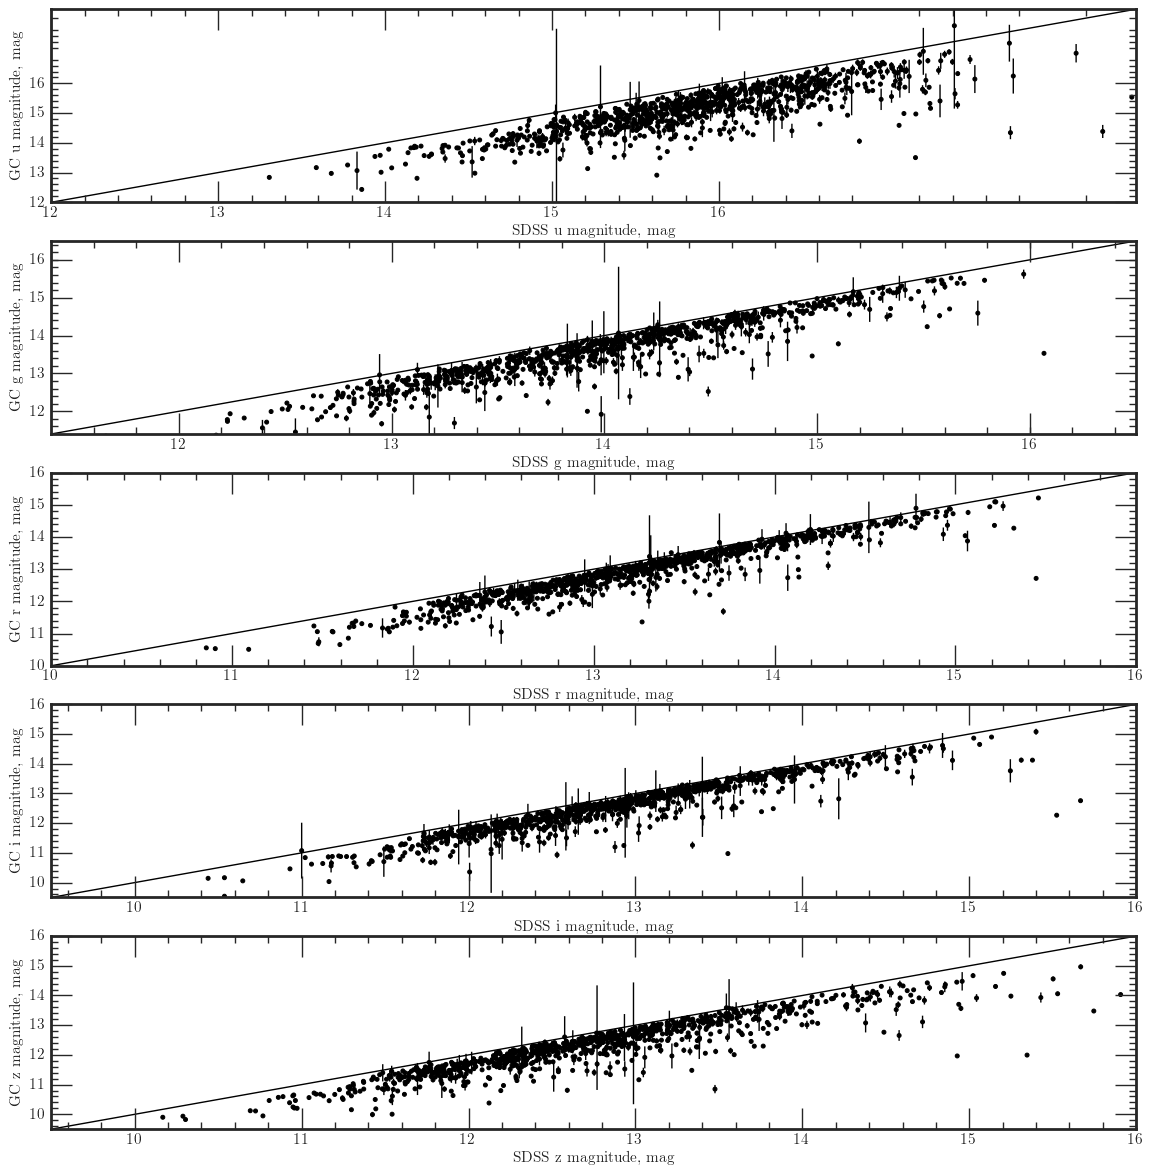
\includegraphics[scale=0.5]{img/all_SDSS_vs_GC}
\caption{Comparison between Petrosian and growth curve u, g, r, i magnitudes}
\label{fig:app_mag_comparison}
\end{figure}

TODO:stellar masses, HLRi, ...
\begin{figure}[h]
\centering
%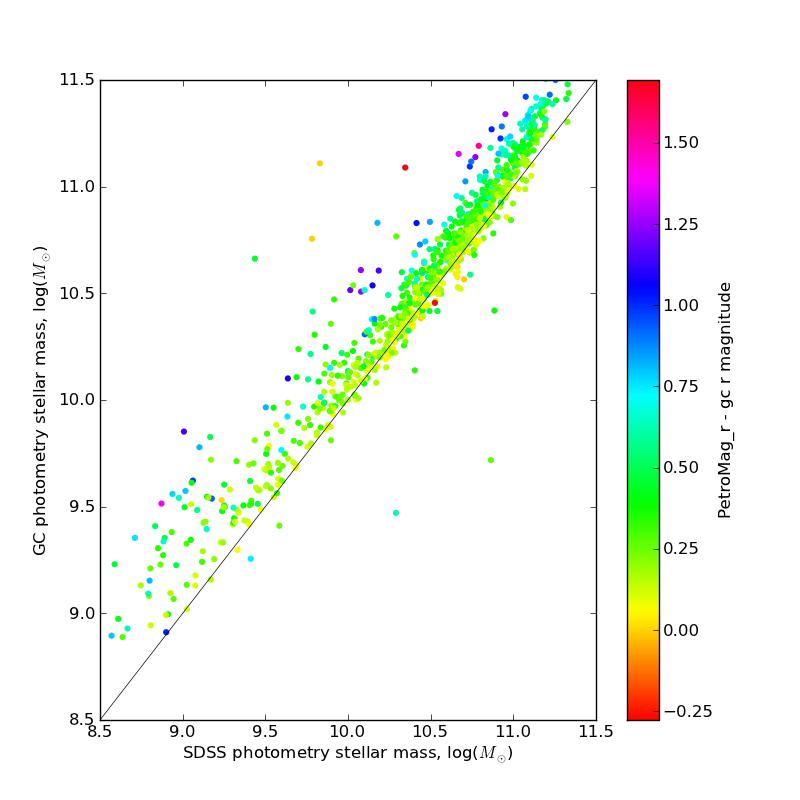
\includegraphics[scale=0.4]{img/st_mass_SDSS_GC_comparison}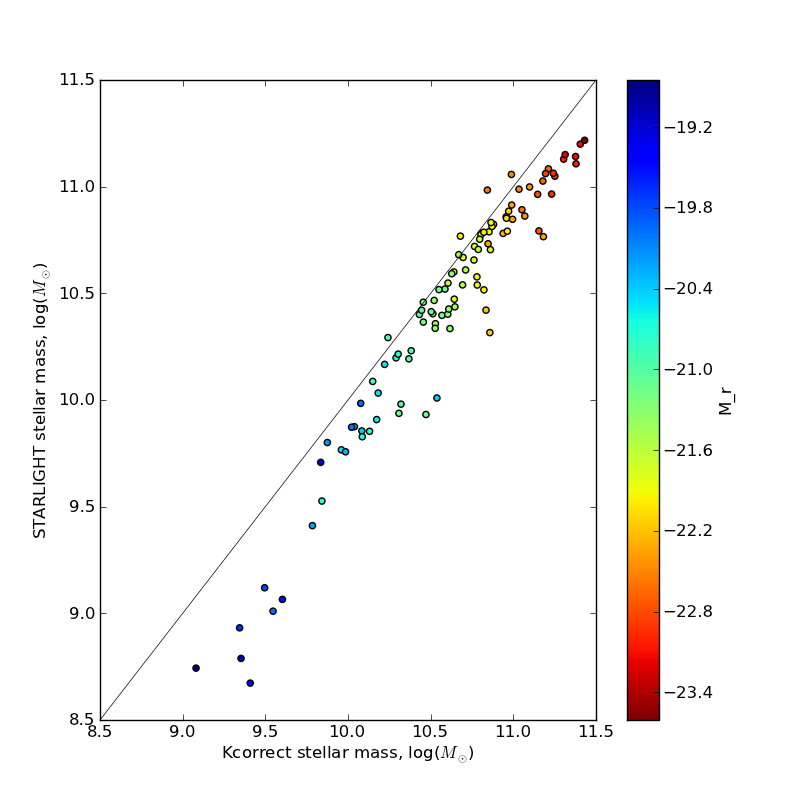
\includegraphics[scale=0.4]{img/st_mass_comparison}
\caption{Left: comparison between kcorrect stellar masses: GC vs. SDSS Petrosian magnitudes. Right: comparison between photometric stellar masses using GC measurements and STARLIGHT stellar masses.}
\label{fig:app_mag_comparison}
\end{figure}

\begin{figure}[h]
\centering
%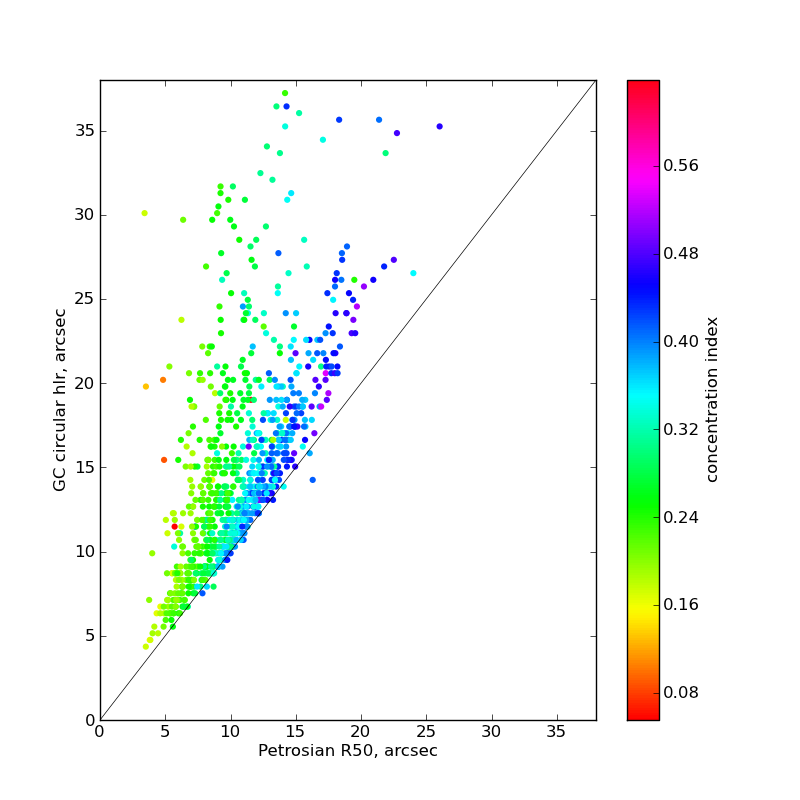
\includegraphics[scale=0.8]{img/petroR50_circ_hlr}
\caption{Petrosian R50 and GC hlr}
\label{fig:petroR50}
\end{figure}




%\begin{figure}[h]
%\centering
%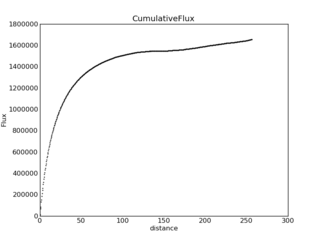
\includegraphics[scale=1]{img/test_noisy_deVauccumulative_Flux-40}
%\caption{Test deVaucouleur galaxy cumulative flux}
%\label{fig:test_cf}
%\end{figure}

\bibliography{phot_bib}
\clearpage\end{document} 
